%!TEX root = ./main.tex
\section{Results}
The results of this research are based on the commits of the three repositories: \textit{Sonarqube}, \textit{Hadoop} and \textit{Elasticsearch}.

\begin{table}[!ht]
\centering
\begin{tabular}{|l|l|}
\hline
\multicolumn{2}{|c|}{Sonarqube} \\ \hline
Amount of monthly metrics commits & 55  \\ \hline
Average amount of evaluated java files & 3170  \\ \hline
Average amount of class-pairs found for each commit & 959 \\ \hline
Percentage class-pairs to total amount of java files & 60\% \\ \hline
Total amount of test refactors found (in last 5 years) & 6832 \\ \hline
\end{tabular}
\caption{Statistics of the mined data of the sonarqube repository}
\label{table:6}
\end{table}

\begin{table}[!ht]
\centering
\begin{tabular}{|l|l|}
\hline
\multicolumn{2}{|c|}{Hadoop} \\ \hline
Amount of monthly metrics commits & 77 \\ \hline
Average amount of evaluated java files & 1466  \\ \hline
Average amount of class-pairs found for each commit & 112 \\ \hline
Percentage class-pairs to total amount of java files & 15\% \\ \hline
Total amount of test refactors found (in last 5 years) & 5452 \\ \hline
\end{tabular}
\caption{Statistics of the mined data of the hadoop repository}
\label{table:7}
\end{table}


\begin{table}[!ht]
\centering
\begin{tabular}{|l|l|}
\hline
\multicolumn{2}{|c|}{Elasticsearch} \\ \hline
Amount of monthly metrics commits & 45  \\ \hline
Average amount of evaluated java files & 3875  \\ \hline
Average amount of class-pairs found for each commit & 237 \\ \hline
Percentage class-pairs to total amount of java files & 16\% \\ \hline
Total amount of test refactors found (in last 4 years) & 10933 \\ \hline
\end{tabular}
\caption{Statistics of the mined data of the elasticsearch repository}
\label{table:8}
\end{table}

The amount of monthly commits are mined over the whole course of the project. The amount of commits might be slightly inconsistent because the months during the course of the projects where nothing was commited. Because of time constraints we were only able to mine the test refactors of the past 4 years of the elasticsearch project.

\subsection{RQ1: What type of refactorings do developers apply on test code?}
\label{refactormethods}
In order to find out what type of refactors developers apply on test code (\textbf{RQ1}), we used refactorminer on multiple repositories to extract all kind of refactors out of the commits. After all the refactors were found, we grouped the refactor methods together and counted them as can be seen in table~\ref{table:9}
\ifx true false

\begin{table}[!ht]
\centering
\begin{tabular}{|l|l|l|l|}
\hline
\multicolumn{4}{|c|}{Sonarqube} \\ \hline
Extract Method & 315 & Pull Up Attribute & 33 \\ \hline
Move Class & 1118 & Extract Superclass & 12 \\ \hline
Move Attribute & 341 & Push Down Method & 37 \\ \hline
Rename Package & 6 &  Push Down Attribute & 3 \\ \hline
Move Method & 553 & Extract Interface & 1 \\ \hline
Inline Method & 53 & Rename Class & 820 \\ \hline
Pull Up Method & 59 & Rename Method & 3481 \\ \hline
\end{tabular}
\caption{Amount of refactorings by type in sonarqube}
\label{table:9}
\end{table}

\begin{table}[!ht]
\centering
\begin{tabular}{|l|l|l|l|}
\hline
\multicolumn{4}{|c|}{Hadoop} \\ \hline
Extract Method & 1690 & Pull Up Attribute & 152 \\ \hline
Move Class & 261 & Extract Superclass & 46 \\ \hline
Move Attribute & 395 & Push Down Method & 2 \\ \hline
Rename Package & 0 &  Push Down Attribute & 0 \\ \hline
Move Method & 721 & Extract Interface & 3 \\ \hline
Inline Method & 89 & Rename Class & 555 \\ \hline
Pull Up Method & 175 & Rename Method & 1363 \\ \hline
\end{tabular}
\caption{Amount of refactorings by type in hadoop}
\label{table:10}
\end{table}

\begin{table}[!ht]
\centering
\begin{tabular}{|l|l|l|l|}
\hline
\multicolumn{4}{|c|}{Elasticsearch} \\ \hline
Extract Method & 565 & Pull Up Attribute & 23 \\ \hline
Move Class & 1363 & Extract Superclass & 73 \\ \hline
Move Attribute & 282 & Push Down Method & 298 \\ \hline
Rename Package & 6 &  Push Down Attribute & 100 \\ \hline
Move Method & 1071 & Extract Interface & 0 \\ \hline
Inline Method & 57 & Rename Class & 2401 \\ \hline
Pull Up Method & 311 & Rename Method & 4370 \\ \hline
\end{tabular}
\caption{Amount of refactorings by type in elasticsearch}
\label{table:11}
\end{table}

\fi

\begin{table}[!ht]
\centering
\begin{tabular}{|l|l|l|l|}
\hline
\multicolumn{4}{|c|}{Sonarqube, Hadoop and Elasticsearch} \\ \hline
Extract Method & 2570 & Pull Up Attribute & 208 \\ \hline
Move Class & 2742 & Extract Superclass & 131 \\ \hline
Move Attribute & 1018 & Push Down Method & 337 \\ \hline
Rename Package & 12 &  Push Down Attribute & 103 \\ \hline
Move Method & 2345 & Extract Interface & 4 \\ \hline
Inline Method & 199 & Rename Class & 3776 \\ \hline
Pull Up Method & 545 & Rename Method & 9214 \\ \hline
\end{tabular}
\caption{Amount of refactorings by type in elasticsearch}
\label{table:9}
\end{table}

\begin{figure}[!ht]
 \centering
 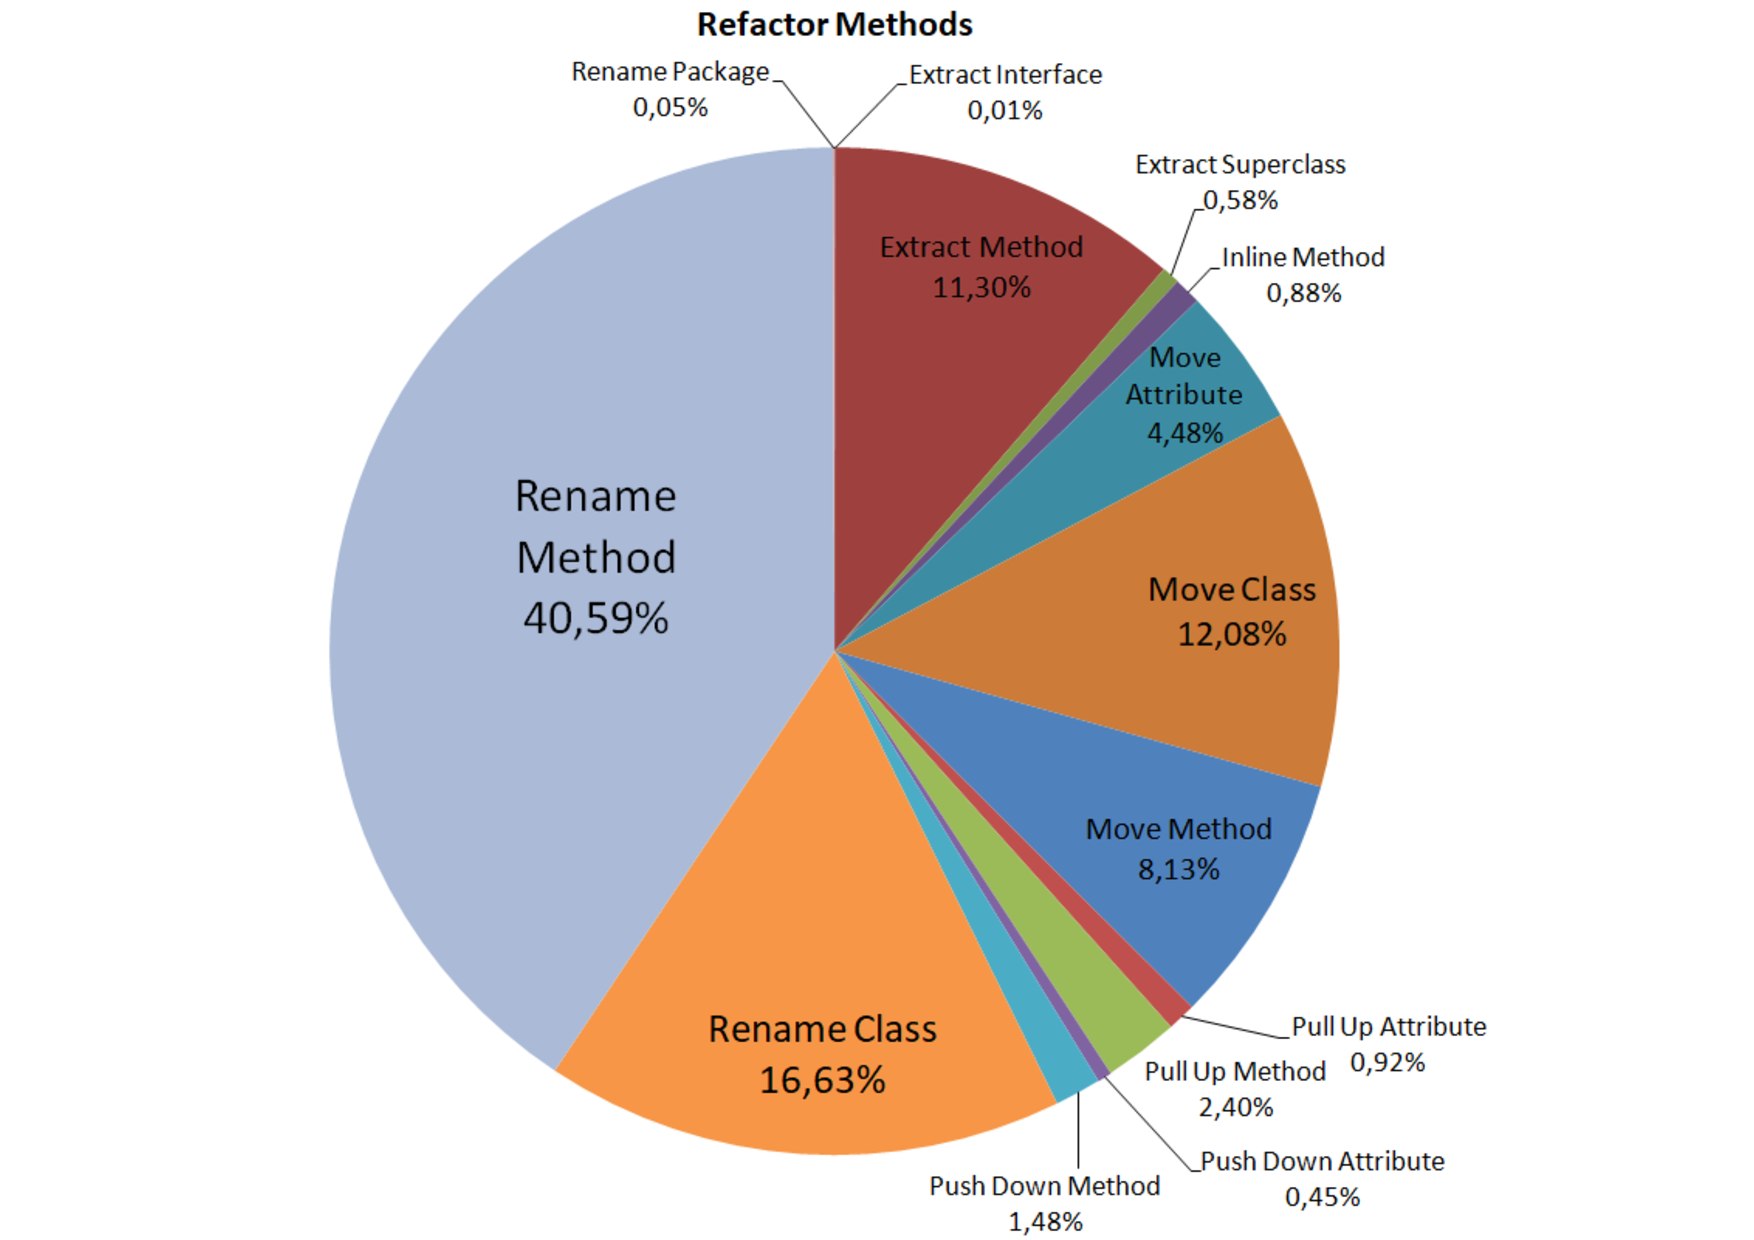
\includegraphics[width=\linewidth]{resources/refactorMethods.pdf}
 \caption{Percentages of the refactor methods of all the repositories}
 \label{figure:piechart}
\end{figure}


After examining the results it was clear that some refactor methods were used more often than others. The most popular refactor method for test code would be \textit{Rename Method}. The refactor methods \textit{Rename Class}, \textit{Move Class} and \textit{Extract Method} were also used a lot. These methods are used for improving the names and location of codes, but also for giving the code a more logical structure. However, because these are all refactors for test files there is a strong possibility that some of these refactors are a result of refactors that are made in the production code. Refactor methods like \textit{Rename Package}, \textit{Extract Interface}, \textit{Extract Superclass}, \textit{Push Down Method} and \textit{Push Down Attribute} were barely used at all. There is also a slight inconsistency in the presented results. Some of the refactor methods were used much more in one of the repositories than the other repositories. For instance, \textit{Extract Method} was used much more in the hadoop repository as in the other two repositories. This cause of this inconsistency might be the case that the developers of each project had their own ideas about refactoring code, however there might also be a slight inconsistency in the classifications of the refactorminer tool.
%In the \textit{Sonarqube} project, the refactor method \textit{Rename Method} seems to be used far more often than in the \textit{Hadoop} project. The same can be said about the refactor method \textit{Extract Method}, which is used far more often in the Hadoop project as in the Sonarqube project. Ofcourse, each project has its own difficulties and thereby their own refactorings. 

%-----------------------------------------------------------------------------------------------
\subsection{RQ2: Does the refactoring of test code affect the maintainability of production code?}\label{maintainability:improved}
In this section we want to adres the results found that have been collected in an attempt to answer RQ2. Refactor data on test classes has been gathered and their matching production classes were checked every 10 commits after that for 5 versions in total, so up to 50 commits ahead. As mentioned in the explanation of RQ2 we will be looking at refactors on test code that significantly improved the maintainability of that test class. We define a significant improvement as a summed difference in the classes each metric among LOC, NOF, NOM and WMC. An example, a class that went from Medium to Low in terms of LOC, has a difference of 1 in terms of LOC. High to Very Low is a difference of 4, Low to High is a difference of -2. Adding the difference for each metric gives us the summed difference, if this value exceeds 4 we say the improvement is significant.  Among all projects we have found the follwing numbers:
\begin{table}[!ht]
    \centering
    \begin{tabular}{|l|l|}
        \hline
        \multicolumn{2}{|c|}{Test refactorings} \\ \hline
        Total & 1756 \\ \hline
        Worsened & 236 \\ \hline
        Unaffected & 824 \\ \hline
        Improved & 696 \\ \hline
        Significantly improved & 108 \\ \hline
    \end{tabular}
    \caption{Counts of test refactorings and how they affected maintainability}
    \label{table:12}
\end{table}
We then check the first and last version of the matching production class that was tracked and calculate the difference here as well. Some production files could not be tracked, this can be accounted to rename or deletions of the file causing our code to be unable to find the file.
\begin{table}[!ht]
    \centering
    \begin{tabular}{|l|l|}
        \hline
        \multicolumn{2}{|c|}{Tracked production files} \\ \hline
        Total & 108 \\ \hline
        Affected & 0 \\ \hline
        Unaffected & 85 \\ \hline
        Error in tracking & 23 \\ \hline
    \end{tabular}
    \caption{Tracked production files' maintainability after significant maintainability improving test refactor}
    \label{table:13}
\end{table}
Surprising not a single production file was modified significantly (i.e. causing a shift in its classification among the metrics we look at). Suggesting that it is very unlikely that a refactoring in test code that significantly improves maintainability causes a similar improvement in the production class under test. Now this result is not what we were expecting, now this is also something that might be related to the projects under analysis, updating test code might not happen before updating the production class, perhaps it is the other way around, production code first, after which test code gets updated. Perhaps it happens more in a periods of pure testing and pure development, such period have also been identified by \cite{zaidman2008mining}. This way our method by looking up to 50 commits in the future after a test code refactoring, does not find the corresponding production file change, if present at all. On the other hand if testing and development are done in different periods then we cannot accredit a test code refactoring to cause a change in production code.

%-----------------------------------------------------------------------------------------------
\subsection{RQ3: What is the correlation between test code maintainability and production code maintainability?}\label{maintainability:correlation}
Using the categories defined in section \ref{ourmaintainabilitymetric} and the class pairs we have extracted from the three projects under analysis we have categorized the risk of each metric for each class in each classpair. Since we have mined the history of the entire project month by month we have chosen to visualise 3 versions evenly distributed over each project's history, hence 9 versions per plot, since visualising all of them would mean showing tens of thousands of datapoints in one plot, making the visualisation look cluttered. By choosing 3 versions evenly over each projects history we still get a good image of the distribution in each projects entire lifetime.

Each datapoint in the plot represents a pair of a test class and the matching production class under test. We see on both axis the risk categories, the X-axis shows the category in which the test class of the pair is in and the Y-axis shows the category in which the production class of the pair is in.

\subsubsection{Analysing the results}
Throughout all the metrics we have analysed in every project we see a strong correlation in production and test classes both being classified in the Very Low risk category. This correlation is not that present in the other categories and this holds for each metric. We do however notice a high density in the leftmost column in each plot. This indicates that where production classes are being classified in a variety of classes (albeit having the most in the Very Low category) where the vast majority of test classes is classified in the Very Low risk category. We think this can be attributed to the general lower complexity of a test class compared to a production class. For example, a highly complex production class can still be tested with a relatively simple test class that verifies if the output of certain functions is as expected.

The high density in the Very Low category for both test and production classes is a surprising result, it seems that for each of these metrics it holds that where a production class is categorised as low risk, so is the corresponding test class, giving an indication that a correlation is present. However that we do not see this density in the Low/Low, Medium/Medium and High/High categories hints that the correlation doesn't hold in all situations. This can however be led back to the argument presented earlier, that even higher complexity classes can be tested using relatively simple test classes.
\begin{figure}
    \centering
    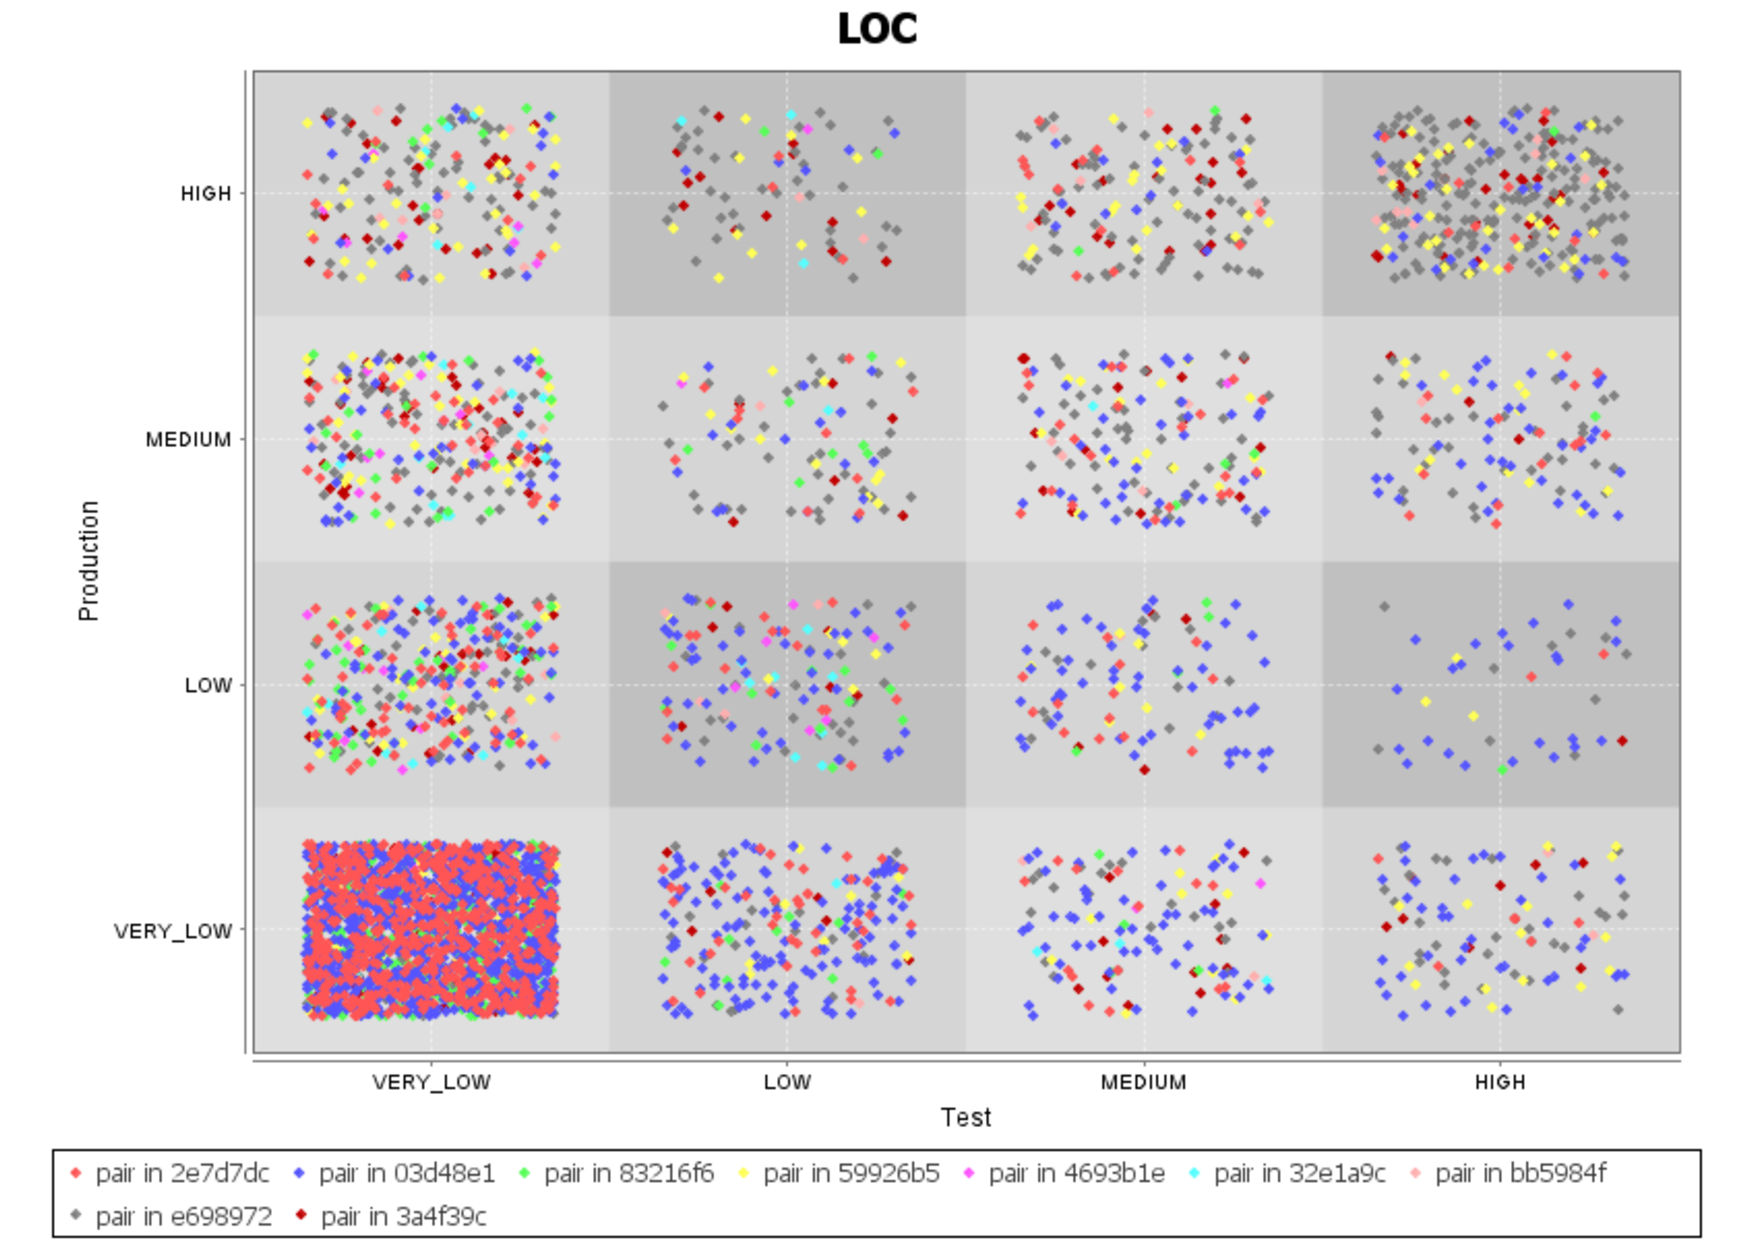
\includegraphics[width=\linewidth]{resources/LOC.pdf}
    \caption{LOC categorization of test-production code class pairs}
    \label{figure:loc}
\end{figure}
\begin{figure}
    \centering
    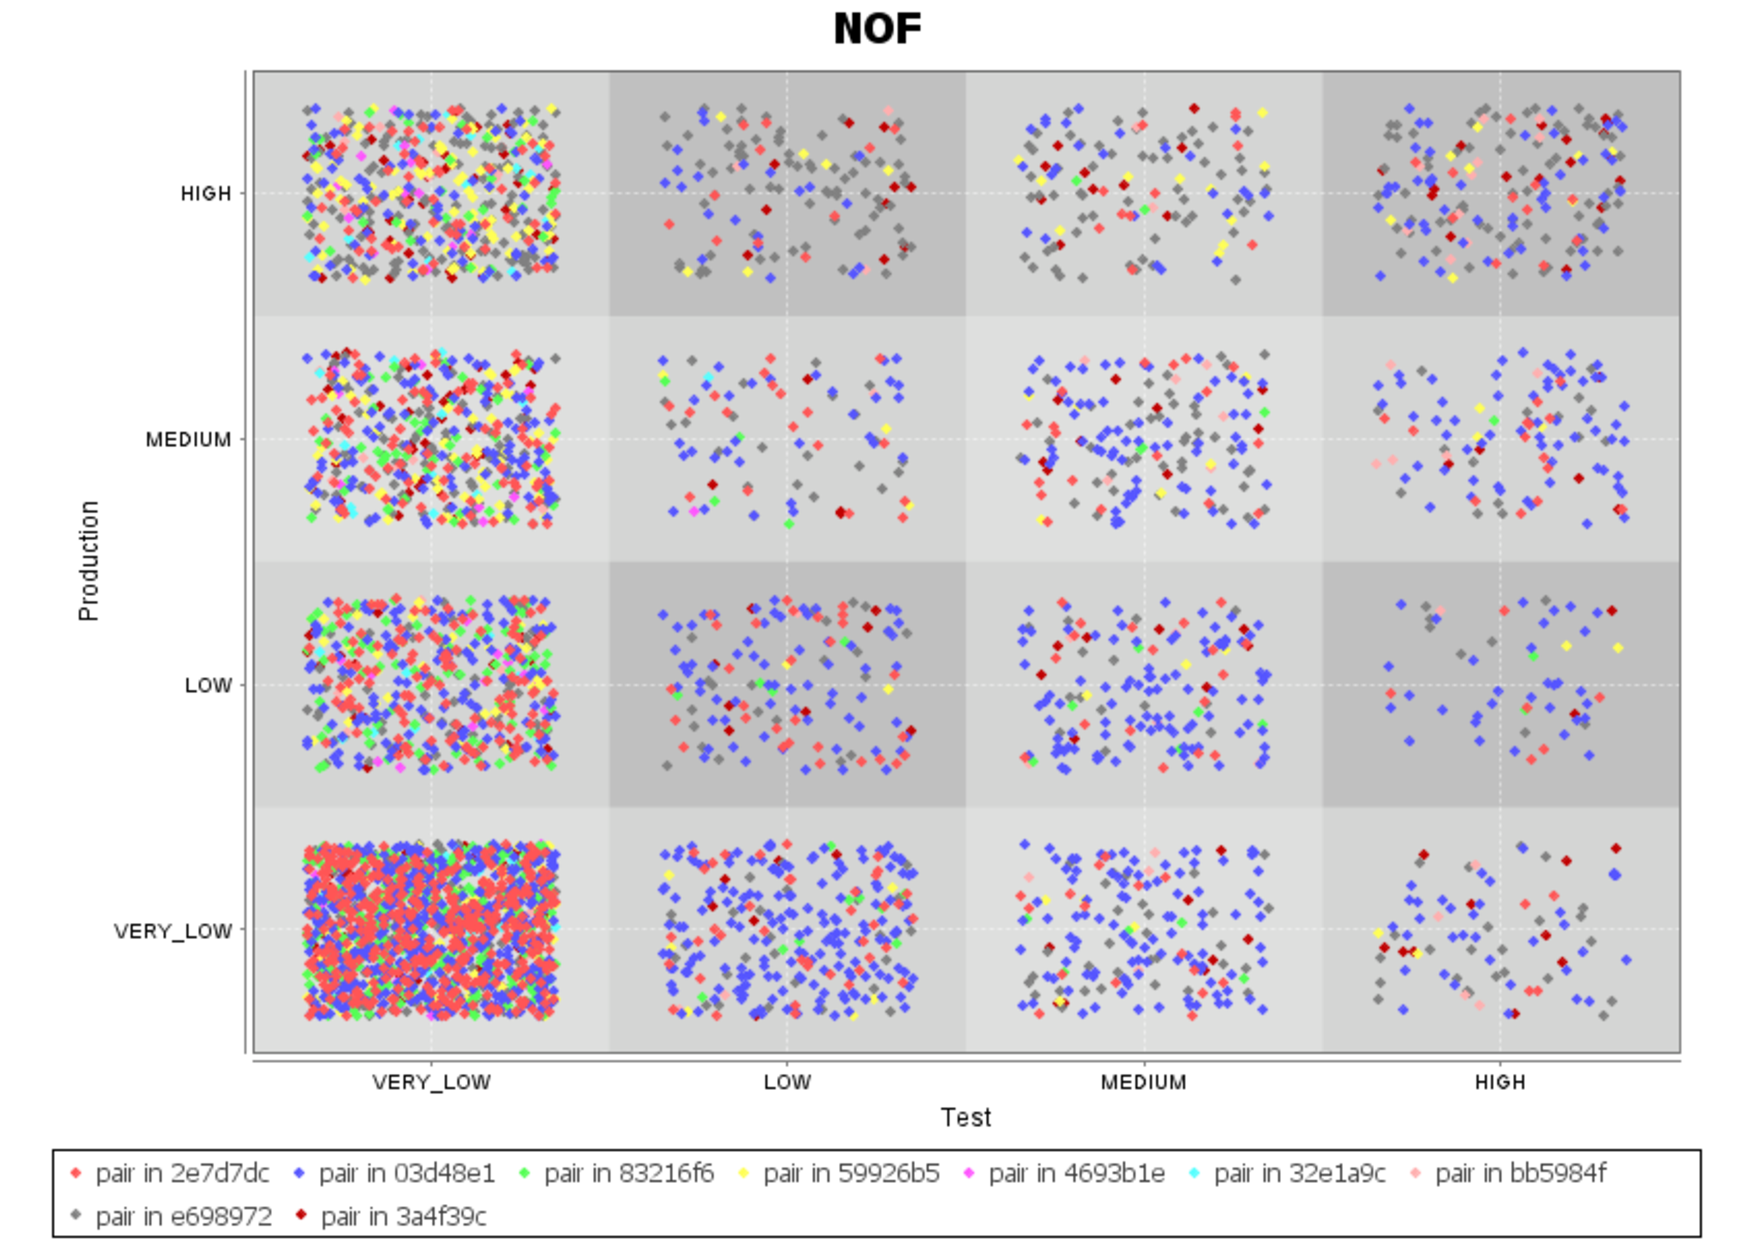
\includegraphics[width=\linewidth]{resources/NOF.pdf}
    \caption{NOF categorization of test-production code class pairs}
    \label{figure:nof}
\end{figure}

\begin{figure}
    \centering
    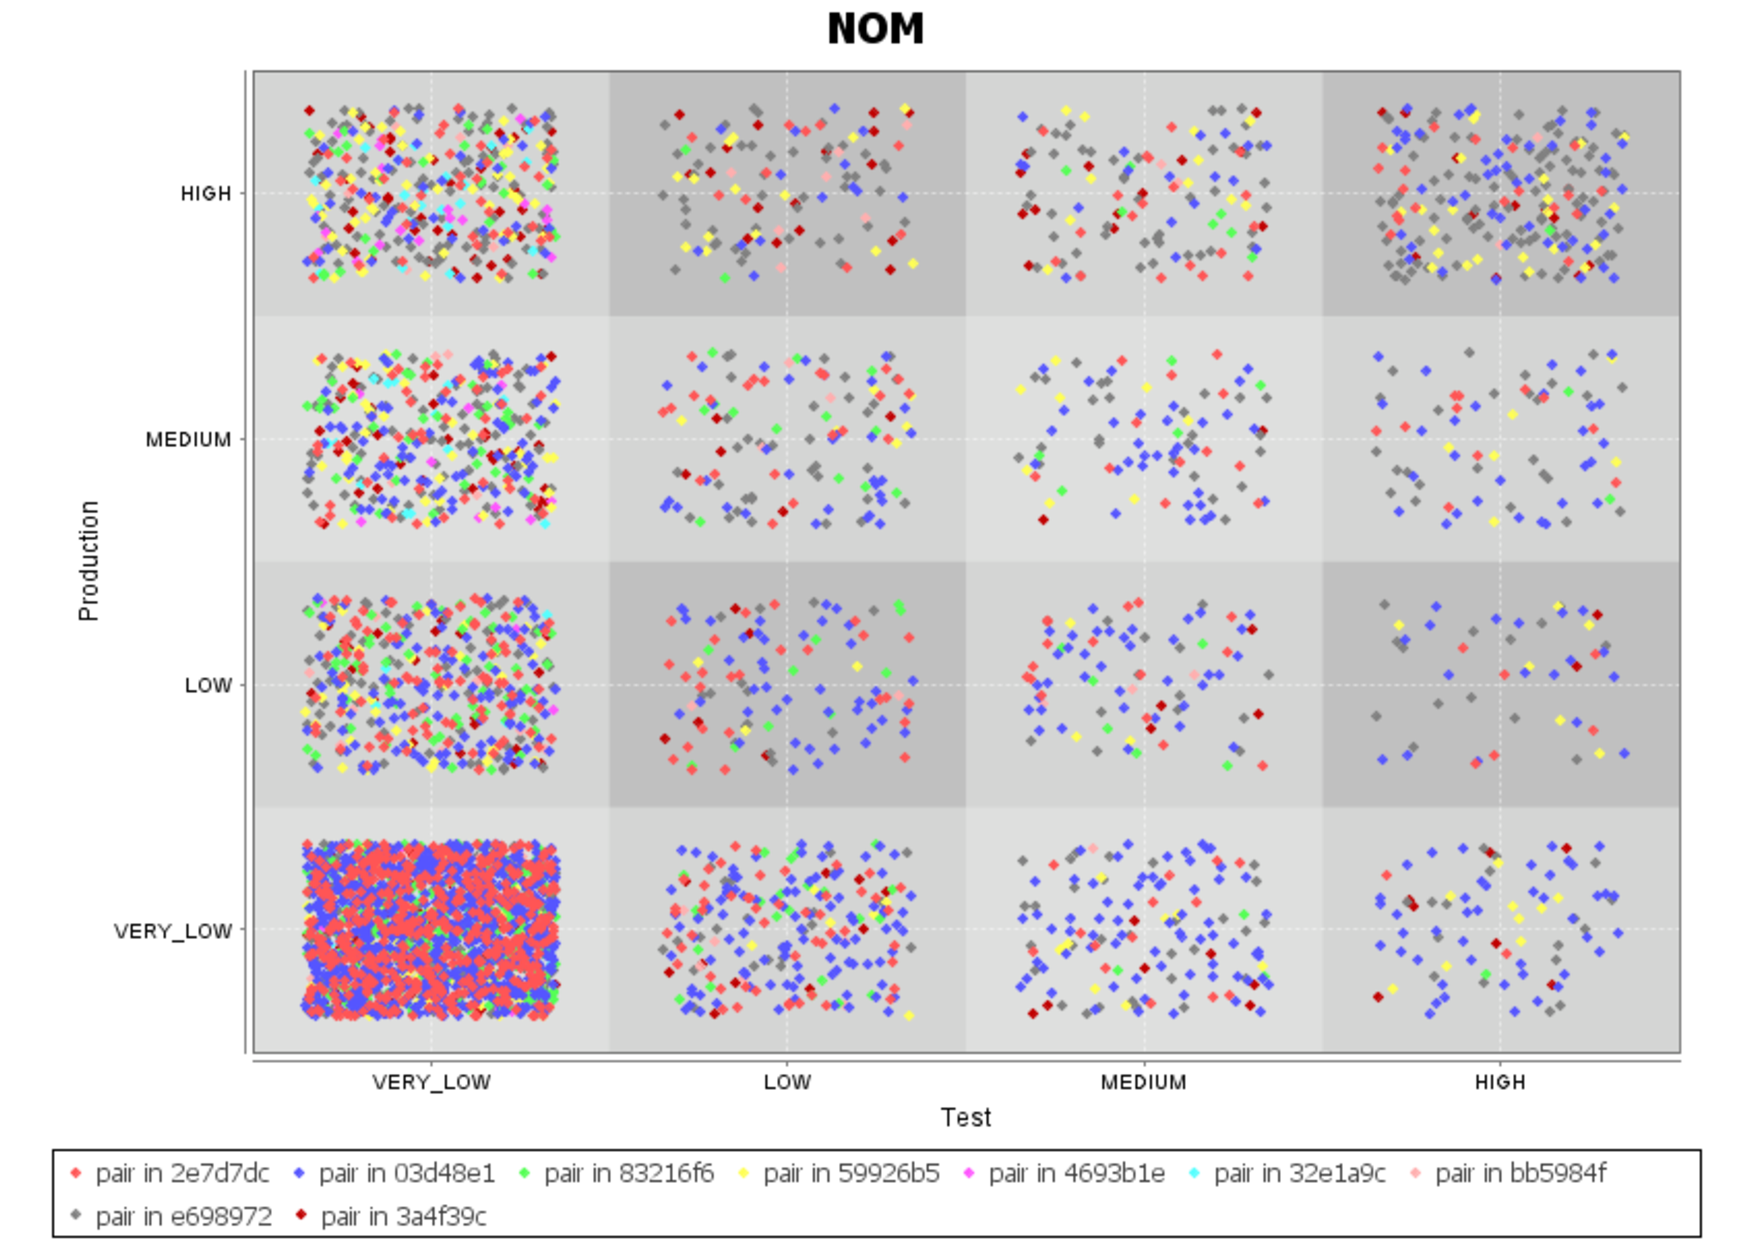
\includegraphics[width=\linewidth]{resources/NOM.pdf}
    \caption{NOM categorization of test-production code class pairs}
    \label{figure:nom}
\end{figure}
\begin{figure}
    \centering
    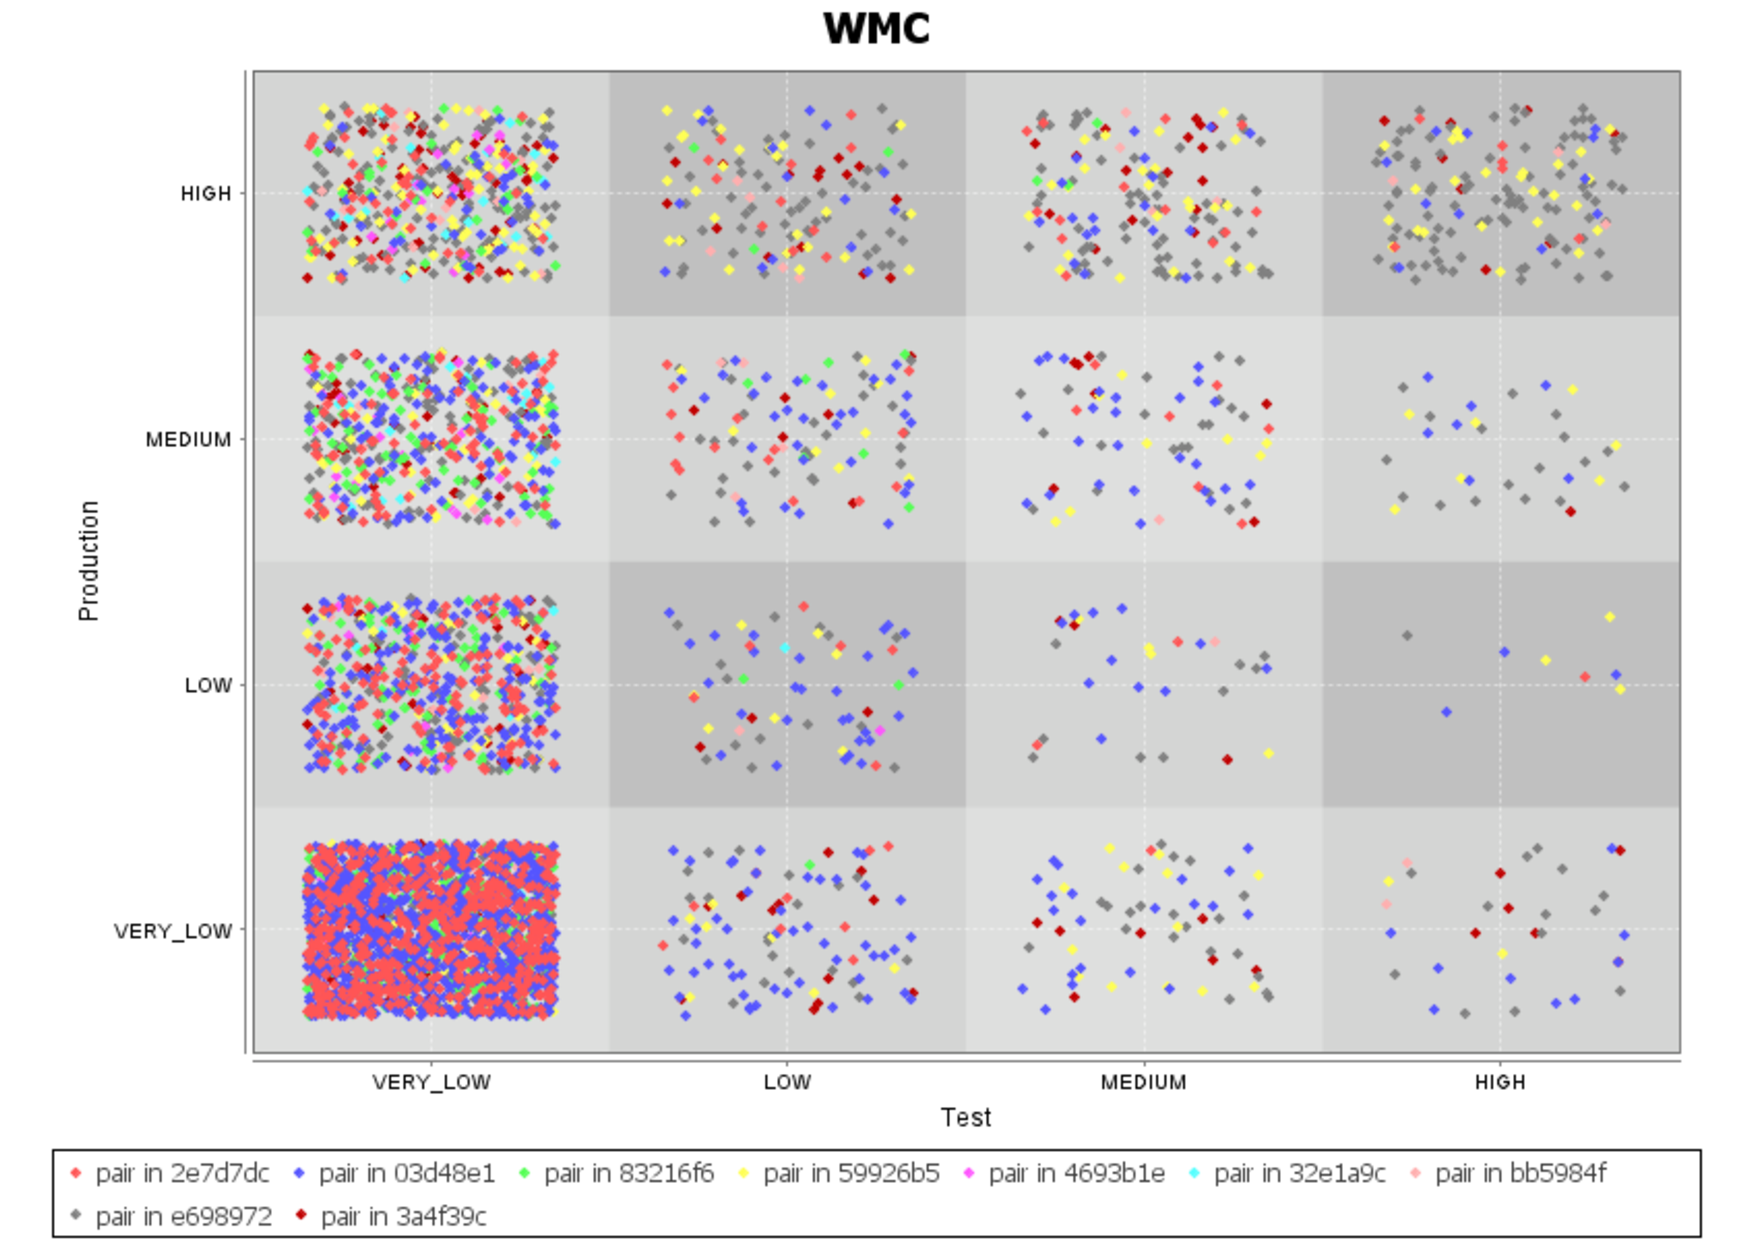
\includegraphics[width=\linewidth]{resources/WMC.pdf}
    \caption{WMC categorization of test-production code class pairs}
    \label{subfigure:wmc}
\end{figure}


